% Options for packages loaded elsewhere
\PassOptionsToPackage{unicode}{hyperref}
\PassOptionsToPackage{hyphens}{url}
%
\documentclass[
]{article}
\usepackage{lmodern}
\usepackage{amssymb,amsmath}
\usepackage{ifxetex,ifluatex}
\ifnum 0\ifxetex 1\fi\ifluatex 1\fi=0 % if pdftex
  \usepackage[T1]{fontenc}
  \usepackage[utf8]{inputenc}
  \usepackage{textcomp} % provide euro and other symbols
\else % if luatex or xetex
  \usepackage{unicode-math}
  \defaultfontfeatures{Scale=MatchLowercase}
  \defaultfontfeatures[\rmfamily]{Ligatures=TeX,Scale=1}
\fi
% Use upquote if available, for straight quotes in verbatim environments
\IfFileExists{upquote.sty}{\usepackage{upquote}}{}
\IfFileExists{microtype.sty}{% use microtype if available
  \usepackage[]{microtype}
  \UseMicrotypeSet[protrusion]{basicmath} % disable protrusion for tt fonts
}{}
\makeatletter
\@ifundefined{KOMAClassName}{% if non-KOMA class
  \IfFileExists{parskip.sty}{%
    \usepackage{parskip}
  }{% else
    \setlength{\parindent}{0pt}
    \setlength{\parskip}{6pt plus 2pt minus 1pt}}
}{% if KOMA class
  \KOMAoptions{parskip=half}}
\makeatother
\usepackage{xcolor}
\IfFileExists{xurl.sty}{\usepackage{xurl}}{} % add URL line breaks if available
\IfFileExists{bookmark.sty}{\usepackage{bookmark}}{\usepackage{hyperref}}
\hypersetup{
  hidelinks,
  pdfcreator={LaTeX via pandoc}}
\urlstyle{same} % disable monospaced font for URLs
\usepackage[margin=1in]{geometry}
\usepackage{graphicx,grffile}
\makeatletter
\def\maxwidth{\ifdim\Gin@nat@width>\linewidth\linewidth\else\Gin@nat@width\fi}
\def\maxheight{\ifdim\Gin@nat@height>\textheight\textheight\else\Gin@nat@height\fi}
\makeatother
% Scale images if necessary, so that they will not overflow the page
% margins by default, and it is still possible to overwrite the defaults
% using explicit options in \includegraphics[width, height, ...]{}
\setkeys{Gin}{width=\maxwidth,height=\maxheight,keepaspectratio}
% Set default figure placement to htbp
\makeatletter
\def\fps@figure{htbp}
\makeatother
\setlength{\emergencystretch}{3em} % prevent overfull lines
\providecommand{\tightlist}{%
  \setlength{\itemsep}{0pt}\setlength{\parskip}{0pt}}
\setcounter{secnumdepth}{-\maxdimen} % remove section numbering
\usepackage{setspace}\doublespacing
\usepackage{lineno}\linenumbers

\author{}
\date{\vspace{-2.5em}}

\begin{document}

\hypertarget{a-standardized-effect-size-for-evaluating-the-strength-of-phylogenetic-signal-and-why-lambda-is-not-appropriate}{%
\section{A Standardized Effect Size for Evaluating the Strength of
Phylogenetic Signal, and Why Lambda is not
Appropriate}\label{a-standardized-effect-size-for-evaluating-the-strength-of-phylogenetic-signal-and-why-lambda-is-not-appropriate}}

\hfill\break

\hypertarget{abstract}{%
\section{Abstract}\label{abstract}}

Macroevolutionary studies frequently characterize the phylogenetic
signal in phenotypes, and wish to compare the strength of that signal
across traits. However, analytical tools for such comparisons have
largely remained underdeveloped. In this study, we evaluated the
efficacy of one commonly used parameter (Pagel's \(\lambda\)) to
estimate the strength of phylogenetic signal in phenotypic traits, and
evaluate the degree to which \(\lambda\) correctly identifies known
levels of phylogenetic signal. We find that the precision of \(\lambda\)
in estimating actual levels of phylogenetic signal is often inaccurate,
and that biological interpretations of the strength of phylogenetic
signal based on \(\lambda\) are therefore compromised. We then propose a
standardized effect size based on \(\kappa\) (\(Z_\kappa\)), which
measures the strength of phylogenetic signal, and places it on a common
scale for statistical comparison. Tests based on \(Z_\kappa\) provide a
mechanism for formally comparing the strength of phylogenetic signal
across datasets, in much the same manner as effect sizes may be used to
summarize patterns in quantitative meta-analysis. Our approach extends
the phylogenetic comparative toolkit to address hypotheses that compare
the strength of phylogenetic signal between various phenotypic traits,
even when those traits are found in different evolutionary lineages or
have different units or scale.

\newpage

\hypertarget{introduction}{%
\section{Introduction}\label{introduction}}

Investigating macroevolutionary patterns of trait variation requires a
phylogenetic perspective, because the shared ancestry among species
violates an assumption of independence among trait values that is common
for statistical tests (Felsenstein 1985; Harvey and Pagel 1991).
Accounting for this evolutionary non-independence is the purview of
\emph{phylogenetic comparative methods} (PCMs): a suite of analytical
tools that condition trends in the data on the phylogenetic relatedness
of observations (e.g., Grafen 1989; Garland and Ives 2000; Rohlf 2001;
Butler and King 2004). The past several decades have witnessed a rapid
expansion in the development of PCMs to address an ever-growing set of
macroevolutionary hypotheses (Martins and Hansen 1997; O'Meara et al.
2006; Revell and Harmon 2008; Beaulieu et al. 2012; Adams 2014b,a; Adams
and Collyer 2018). These methods are predicated on the notion that
phylogenetic signal -- the tendancy for closely related species to
display similar trait values -- is present in cross-species datasets
(Felsenstein 1985; Pagel 1999; Blomberg et al. 2003). Indeed, under
numerous evolutionary models, phylogenetic signal is to be expected, as
stochastic character change along the hierarchical structure of the tree
of life generates trait covaration among related taxa (see Felsenstein
1985; Blomberg et al. 2003; Revell et al. 2008). \hfill\break

Several analytical tools have been developed to quantify phylogenetic
signal in phenotypic datasets, including measures of serial independence
(\(\mathbf{C}\): Abouheif 1999), autocorrelation estimates (\(I\):
Gittleman and Kot 1990), statistical ratios of trait variation relative
to what is expected given the phylogeny (\(\kappa\): Blomberg et al.
2003; Adams 2014a), and scaling parameters used in maximum likelihood
fitting of the data to the phylogeny (\(\lambda\): Pagel 1999), among
others (e.g., Klingenberg and Gidaszewski 2010). The statistical
properties of these methods -- namely type I error rates and power --
have also been investigated to determine when phylogenetic signal can be
detected and under what conditions (e.g., Münkemüller et al. 2012;
Pavoine and Ricotta 2012; Diniz-Filho et al. 2012; Adams 2014a;
Molina-Venegas and Rodríguez 2017; see also Revell et al. 2008; Revell
2010). One of the most widely used methods for characterizing
phylogenetic signal in macroevolutionary studies is Pagel's \(\lambda\)
(Pagel 1999). The (\(\lambda\)) parameter transforms the lengths of the
internal branches of the phylogeny to improve a fit of data to the
phylogeny via maximum likelihood (Pagel 1999; Freckleton et al. 2002).
Pagel's \(\lambda\) ranges from \(0\to1\), with larger values signifying
a greater dependence of observed trait variation on the phylogeny.
Pagel's \(\lambda\) also has the appeal that it may be included in
phylogenetic generalized least-squares regression (PGLS) to account for
the degree of phylogenetic signal in comparative analyses (see
Freckleton et al. 2002). \hfill\break 

In addition to functioning as a parameter that is tuned for appropriate
analysis, \(\lambda\) can function as a descriptive statistic to
describe the relative strength of phylogenetic signal in phenotypic
traits, to determine the extent to which shared evolutionary history has
influenced trait covariation among taxa. The appeal of \(\lambda\) as a
descriptive statistic for evolutionary biologists is a basis for
interpreting ``weak'' versus ``strong'' phylogenetic signal; i.e., small
versus large values of \(\lambda\), respectively, in a comparative sense
(e.g., De Meester et al. 2019; Pintanel et al. 2019; Su et al. 2019).
Indeed, statements regarding the strength of phylogenetic signal based
on \(\lambda\) are rather common in the evolutionary literature. For
instance, of the 204 papers published in 2019 that estimated and
reported Pagel's \(\lambda\) (found from a literature survey we
conducted in Google.scholar), 40\% interpreted the strength of
phylogenetic signal for at least one phenotypic trait. Further, because
nearly half of the 1,572 \(\lambda\) values reported were near 0 or 1
(Figure 1) where the biological interpretation of \(\lambda\) is known,
this percentage is even higher. \hfill\break

{[}insert Figure 1 here{]} \hfill\break

Various other approaches use \(\lambda\) as a parameter that can be
varied for inferences akin to sensitivity analysis. For instance, some
have performed likelihood ratio tests that compare observed model fits
to those obtained when \(\lambda=0\) or \(\lambda=1\) (Freckleton et al.
2002; Cooper et al. 2010; Bose et al. 2019) or evaluated whether
observed \(\lambda\) differs from an expected \(\lambda\), based on
confidence intervals generated for the expected value (Vandelook et al.
2019). Qualitative comparisons of \(\lambda\) estimates have also been
performed for multiple traits on the same phylogenetic tree to infer
whether the strength of phylogenetic signal is greater in one trait as
compared to another (e.g., Liu et al. 2019; Bai et al. 2019).
\hfill\break

It seems intuitive to interpret the strength of phylogenetic signal
based on the value of \(\lambda\), as \(\lambda\) is a parameter on a
bounded scale (\(0\to1\)) for which interpretation of its extremal
points are understood. Specifically, \(\lambda=0\) represents no
phylogenetic signal, while \(\lambda=1\) is phylogenetic signal as
expected under Brownian motion. However, equating values of \(\lambda\)
directly to the strength of phylogenetic signal presumes two important
statistical properties that have not been fully explored. First, it
presumes that values of \(\lambda\) can be precisely estimated, as
biological inferences regarding the strength of phylogenetic signal
depend on high accuracy in its estimation. Therefore, understanding the
precision in estimating \(\lambda\) is paramount. One study (Boettiger
et al. 2012) found that estimates of Pagel's \(\lambda\) displayed less
variation (i.e., greater precision) when data were simulated on a large
phylogeny (\(N=281\)) as compared to a small one (\(N=13\)). From this
observation it was concluded that insufficient data (i.e., the number of
species) was the underlying cause of the increased variation across
parameter estimates (Boettiger et al. 2012). Indeed, such a pattern is
common with statistical estimators, as summary statistics and parameters
are often more precise at greater sample sizes (Cohen 1988). However,
this conclusion also implies that the precision of \(\lambda\) remains
constant across its range (\(\lambda = 0 \to 1\)); an assumption that to
date, has not been verified. Thus, despite widespread use of Pagel's
(1999) \(\lambda\) in macroevolutionary studies, at present, we lack a
general understanding of the precision with which \(\lambda\) can
estimate levels of phylogenetic signal in phenotypic datasets.
\hfill\break

Second, while estimates of \(\lambda\) are within a bounded scale
(\(0\to1\)), this does not \emph{de-facto} imply that the estimated
values of this parameter correspond to the actual strength of the
underlying input signal in the data. For this to be the case,
\(\lambda\) must be a statistical effect size. Effect sizes are a
measure of the magnitude of a statistical effect in data, represented on
a common scale (Glass 1976; Cohen 1988). Effect sizes have widespread
use in many areas of the quantiative sciences, as they represent
measures that may be readily summarized across datasets as in
meta-analyses (Glass 1976; Hedges and Olkin 1985; Arnqvist and Wooster
1995), or compared among datasets (e.g., Adams and Collyer 2016, 2019a).
Unfortunatley, not all model parameters and descriptive statistics are
effect sizes, and thus many summary measures must first be converted to
statistics with standardized units (i.e., conversion to an effect size)
for meaningful comparison (see Rosenthal 1994). As a consequence, it
follows that only if \(\lambda\) is a statistical effect size can
comparisons of estimates across datasets be interpretable. For the case
of \(\lambda\), this has not yet been explored. \hfill\break

In this study, we evaluate the precision of Pagel's \(\lambda\) for
estimating known levels of phylogenetic signal in phenotypic data. We
use computer simulations with differing numbers of species, differently
shaped phylogenies, and differing input levels of phylogenetic signal,
to explore the degree to which \(\lambda\) correctly identifies known
levels of phylogenetic signal, and under what circumstances. We find
that estimates of \(\lambda\) vary widely for a given input value of
phylogenetic signal, and that the precision in estimating \(\lambda\) is
not constant across its range. Rather, there is decreased precision when
input levels of phylogenetic signal are of intermediate strength.
Additionally, the same estimated values of \(\lambda\) may be obtained
from datasets containing vastly different input levels of phylogenetic
signal. Thus, \(\lambda\) is not a reliable indicator of the strength of
phylogenetic signal in phenotypic data. We then describe a standardized
effect size for measuring the strength of phylogenetic signal in
phenotypic datasets, and apply the concept to two common measures of
phylogenetic signal: \(\lambda\) and \(\kappa\). Through simulations we
find that the precision of effect sizes based on \(\lambda\)
(\(Z_{\lambda}\)) are less reliable than that those based on \(\kappa\)
(\(Z_\kappa\)), implying that \(Z_\kappa\) is a more robust effect size
measure. We also propose a two-sample test statistic that may be used to
compare the strength of phylogenetic signal among datasets, and provide
an empirical example to demonstrate its use. We conclude that estimates
of phylogenetic signal using Pagel's \(\lambda\) are often inaccurate,
and thus interpreting strength of phylogenetic signal in phenotypic
datasets based on this measure is compromised. By contrast, effect sizes
obtained from \(\kappa\) hold promise for characterizing phylogenetic
signal, and for comparing the strength of phylogenetic signal across
datasets.

\hypertarget{methods-and-results}{%
\section{Methods and Results}\label{methods-and-results}}

\hypertarget{the-precision-of-lambda-is-variable}{%
\subsection{\texorpdfstring{\emph{The Precision of \(\lambda\) is
Variable}}{The Precision of \textbackslash lambda is Variable}}\label{the-precision-of-lambda-is-variable}}

We conducted a series of computer simulations to evaluate the precision
of Pagel's \(\lambda\). Our primary simulations were based on pure-birth
phylogenies; however, we also evaluated patterns on both balanced and
pectinate trees to determine whether tree shape affected our findings
(see Supporting Information). First we generated 50 pure-birth
phylogenies at each of six different tree sizes, ranging from 32 to 1024
taxa (\(n=2^5 - 2^{10}\)). Next, we rescaled the simulated phylogenies
by multiplying the internal branches by \(\lambda_{in}\), using 21
intervals of 0.05 units across its range
(\(\lambda_{in} = 0.0 \to 1.0\)), resulting in 1050 scaled phylogenies
at each level of species richness (\(n\)). Continuous traits were then
simulated on each phylogeny under a Brownian motion model of evolution
to obtain datasets with differing levels of phylogenetic signal, that
ranged from no phylogenetic signal (when \(\lambda_{in} =0\)), to
phylogenetic signal reflecting Brownian motion (when
\(\lambda_{in} =1\)). For each dataset we then estimated phylogenetic
signal (\(\lambda_{est}\)), and calculated the variance of \(\lambda\)
(\(\sigma^2_\lambda\)) across datasets at each input level of
phylogenetic signal and level of species richness as an estimate of
precision. We verified that the variance of traits simulated had no
effect on phylogenetic signal estimation. \hfill\break

We also evaluated the precision of \(\lambda\) when estimated in PGLS
regression and ANOVA (i.e., \(Y\sim{X}\)). Here, an independent variable
\(X\) was simulated on each rescaled phylogeny under a Brownian motion
model of evolution (for PGLS regression). For phylogenetic ANOVA, random
groups (\(X\)) were obtained by simulating a discrete (binary, 0 or 1)
character on each phylogeny. Next, the dependent variable was simulated
in such a manner as to contain a known relationship with \(X\) plus
random error containing phylogenetic signal. This was accomplished as:
\(Y=\beta{X}+\epsilon\). The association between \(Y\) and \(X\) was
modeled using a range of values: \(\beta=(0.0,0.25, 0.5, 0.75,1.0)\),
and the residual error (\(\epsilon\)) was modeled to contain
phylogenetic signal simulated under a Brownian motion model of evolution
on each rescaled phylogeny:
\(\epsilon=\mathcal{N}(\mu=0,\sigma=\sigma^2\mathbf{C})\): (see Revell
2010 for a similar simulation design). The fit of the phylogenetic
regression was estimated using maximum likelihood, and parameter
estimates (\(\beta_{est}\) and \(\lambda_{est}\)) were obtained. We then
calculated precision estimates (\(\sigma^2_\lambda\)) at each input
level of phylogenetic signal and level of species richness. We verified
that the amount of residual variance simulated had no effect on
\(\sigma^2_\lambda\) but did influence the precision of coefficients
estimated from the linear model (precision increased with smaller
\(\epsilon\), as expected). \hfill\break

All analyses were performed in R v3.6.0 (R Core Team 2019) using the
packages \texttt{geiger} (Harmon et al. 2008), \texttt{caper} (Orme et
al. 2013), \texttt{phytools} (Revell 2012), and \texttt{geomorph} 3.2.1
(Adams and Otárola-Castillo 2013; Adams et al. 2020). R-scripts are
found in the Supporting Information. \hfill\break

\emph{Results.} We found that the precision of \(\lambda_{est}\) varied
widely across simulation conditions. Predictably, precision improved as
the number of species increased (Figure 2). This confirmed earlier
findings of Boettiger et al.~(2012), and adhered to parametric
statistical theory. However, in many cases the set of \(\lambda_{est}\)
spanned nearly the entire range of possible values (e.g., \(n=32\);
\(\lambda_{in}=0.5\): \(\lambda_{est}= 0.0\to 0.985\)), revealing that
estimates of \(\lambda\) were not a reliable indicator of input
phylogenetic signal. Importantly, the precision of \(\lambda_{est}\) was
not uniform across all levels of phylogenetic signal. The worst
precision was observed at intermediate levels of phylogenetic signal
(\(\lambda_{in}\approx0.5\)), while precision improved as input levels
approached the extremes of \(\lambda\)'s range (i.e.,
\(\lambda_{in}\rightarrow0\) \& \(\lambda_{in}\rightarrow1\)). Thus,
estimates of \(\lambda\) were least reflective of the true input signal
at intermediate values. Additionally, even at large levels of species
richness, we found that the range of \(\lambda_{est}\) still encompassed
a substantial portion of possible values (e.g., \(n=512\);
\(\lambda_{in}=0.5\): \(\lambda_{est} = 0.32\to 0.68\)). Likewise, the
same \(\lambda_{est}\) could be obtained from datasets containing vastly
different input levels of phylogenetic signal (e.g., \(n=512\);
\(\lambda_{est} = 0.5\); \(\lambda_{in} = 0.25 \to 0.65\)). These
findings were particularly unsettling when considered in light of our
literature survey. Over one quarter of the \(\lambda\) estimates
published in empirical studies (421 of 1,572) were between
\(\lambda=0.25\) and \(\lambda=0.75\) (Figure 1). This range reflected
the region that our simulations identified as being the least reliable
in terms of accurately characterizing levels of phylogenetic signal, yet
30\% of these mid-range empirical estimates were explicitly interpreted
in terms of the strength of phylogenetic signal that they represented
(i.e., weak, intermediate, strong phylogenetic signal). \hfill\break

Finally, when \(\lambda\) was co-estimated with regression parameters in
PGLS regression and ANOVA, the results of our simulations were quite
similar. Regression parameters (\(\beta\)) were accurately estimated,
confirming earlier findings of Revell (2010) (see Supporting
Information). However, estimates of phylogenetic signal (\(\lambda\))
were less precise (Figure 3; see also Supporting Information), and the
spread of \(\lambda_{est}\) was similar to that observed when
\(\lambda\) was estimated for only the dependent variable, as in Figure
2. Taken together, these findings reveal that \(\lambda_{est}\) does not
precisely characterize observed levels of phylogenetic signal in
phenotypic datasets, and that biological interpretations of the strength
of phylogenetic signal based on \(\lambda\) may be highly inaccurate.
\hfill\break

{[}insert Figure 2 here{]} \hfill\break

{[}insert Figure 3 here{]} \hfill\break 

\hypertarget{a-standardized-effect-size-for-phylogenetic-signal}{%
\subsection{\texorpdfstring{\emph{A Standardized Effect Size for
Phylogenetic
Signal}}{A Standardized Effect Size for Phylogenetic Signal}}\label{a-standardized-effect-size-for-phylogenetic-signal}}

The results above demonstate that \(\lambda\) is not a reliable estimate
of the phylogenetic signal in phenotypic data. As such, biological
interpretations of the strength of phylogenetic signal, and comparisons
of the magnitude of such effects across datasets are severely
compromised when based on this parameter. As an alternative, we propose
that summary estimates of phylogenetic signal be converted to effect
sizes for interpretation and comparison of the relative strength of
phylogenetic signal in phenotypic datasets. Statistically, a
standardized effect size may be found as:

\begin{align}
    Z_{\theta}=\frac{\theta_{obs}-E(\theta)}{\sigma_\theta}
\end{align}

where \(\theta_{obs}\) is the observed test statistic, \(E(\theta)\) is
its expected value under the null hypothesis, and \(\sigma_\theta\) is
its standard error (Glass 1976; Cohen 1988; Rosenthal 1994).
\(Z_{\theta}\) expresses the magnitude of the effect in \(\theta_{obs}\)
by transforming the original test statistic to its standard normal
deviate (Glass 1976; Kelley and Preacher 2012). Typically,
\(\theta_{obs}\) and \(\sigma_\theta\) are estimated from the data,
while \(E(\theta)\) is obtained from the distribution of \(\theta\)
derived from parametric theory. However, recent advances in resampling
theory (Collyer et al. 2015; Adams and Collyer 2016, 2019a; Collyer and
Adams 2018) have shown that \(E(\theta)\) and \(\sigma_\theta\) may also
be obtained from an empirical sampling distribution of \(\theta\)
obtained from permutation procedures. \hfill\break

Adams and Collyer (2019b) suggested that the strength of phylogenetic
signal could be represented as an effect size based on the \(\kappa\)
statistic and its empirical sampling distribution from permutation. Here
we formalize that suggestion, resulting in an effect size of:

\begin{align}
    Z_\kappa=\frac{log(\kappa_{obs})-\hat\mu_{log(\kappa)}}{\hat\sigma_{log(\kappa)}}
\end{align}

where \(\kappa_{obs}\) is the observed phylogenetic signal, and
\(\hat\mu_\kappa\) and \(\hat\sigma_\kappa\) are the mean and standard
deviation of the empirical sampling distribution of \(log(\kappa)\)
obtained via permutation. Note that the logarithm was used because
\(\kappa\) takes only positive values (\(0\to\infty\)) and its sampling
distribution is log-normally distributed (for a similar transformation
when calculating multivariate effect sizes see: Appendix 1 of Collyer
and Adams 2018). \hfill\break

An effect size based on \(\lambda\) could be envisioned, which is found
as:

\begin{align}
    Z_{\lambda}=\frac{\lambda_{obs}-0}{\hat\sigma_\lambda}.
\end{align}

In this case, \(\lambda_{obs}\) and \(\hat\sigma_\lambda\) are
empirically derived using maximum likelihood, as permutation approaches
have not been developed for evaluating \(\lambda\). Note also that under
the null hypothesis, no phylogenetic signal is expected (Freckleton et
al. 2002), and thus \(E(\lambda)=0\) under this condition. \hfill\break

To evaluate the utility of \(Z_\kappa\) and \(Z_\lambda\) we calculated
both effect sizes for the simulated datasets generated above, and
summarized the precision of each using its variance
(\(\sigma^2_{Z_\kappa}\) and \(\sigma^2_{Z_\lambda}\), Figure 4:
additional results in the Supporting Information). Here two things are
evident. First, estimates of \(Z_\kappa\) linearly track the input
phylogenetic signal whereas estimates of \(Z_\lambda\) do not (Figure
4A, B). Thus, actual changes in the strength of phylogenetic signal are
reflected more evenly in the corresponding values of the effect size
\(Z_\kappa\). Second, the precision of \(Z_\kappa\) is considerably more
stable as compared with \(Z_\lambda\). This may be seen by calculating
the coefficients of variation for the set of precision estimates (i.e.,
\(\sigma^2_{Z_\kappa}\) and \(\sigma^2_{Z_\lambda}\)) across input
levels of phylogenetic signal. Coefficients of variation in the
precision of \(Z_\kappa\) were up to an order of magnitude smaller for
than for \(Z_\lambda\) (Figure 4C), implying that estimates of the
strength of phylogenetic signal were more reliable and robust when using
\(Z_\kappa\). \hfill\break

{[}insert Figure 4 here{]}

\hypertarget{statistical-comparisons-of-phylogenetic-signal}{%
\subsection{\texorpdfstring{\emph{Statistical Comparisons of
Phylogenetic
Signal}}{Statistical Comparisons of Phylogenetic Signal}}\label{statistical-comparisons-of-phylogenetic-signal}}

Once the magnitude of phylogenetic signal is characterized using
\(Z_\kappa\), one may wish to compare such measures across datasets, to
determine whether the strength of phylogenetic signal is significantly
greater in one phenotypic trait than another. As with other effect sizes
derived from permutation distributions (e.g., Adams and Collyer 2016,
2019a), a two-sample test statistic may be calculated as:

\begin{align}
  \hat{Z}_{12}=\frac{\lvert{(\kappa_{1}-\hat\mu_{\kappa_1})-(\kappa_{2}-\hat\mu_{\kappa_2})}\rvert}{\sqrt{\hat\sigma^2_{\kappa_1}+\hat\sigma^2_{\kappa_2}}} = \frac{\lvert Z_{\kappa_1} - Z_{\kappa_2}\rvert}{\sqrt{2}}
\end{align}

where \(\kappa_1\), \(\kappa_2\), \(\hat\mu_{\kappa_1}\),
\(\hat\mu_{\kappa_2}\), \(\hat\sigma_{\kappa_1}\), and
\(\hat\sigma_{\kappa_2}\) are as defined above for equation 2. The right
side of the equation illustrates that if \(Z_\kappa\) has already been
calculated for two sampling distributions as in equation 2, the sampling
distributions have unit variance for each of the \(Z_\kappa\)
statistics. Estimates of significance of \(\hat{Z}_{12}\) may be
obtained from a standard normal distribution. Typically,
\(\hat{Z}_{12}\) is considered a two-tailed test, however directional
(one-tailed) tests may be specified should the empirical situation
require it (see Adams and Collyer 2016, 2019a). \hfill\break

\hypertarget{empirical-example}{%
\subsection{\texorpdfstring{\emph{Empirical
Example}}{Empirical Example}}\label{empirical-example}}

To demonstrate the utility of \(\hat{Z}_{12}\) we quantified and
compared the strength of phylogenetic signal of two phenotypic traits
across species of plethodontid salamander. The data were part of a
series of studies examining macroevolutionary trends in phenotypic
diversification in this group (Baken and Adams 2019; Baken et al. 2020).
Our dataset contained surface area to volume ratios (SA:V) and relative
body width (\(\frac{BW}{SVL}\)) for 305 species (Figure 5A). For SA:V,
11 linear body measurements from 2,781 individuals were taken, from
which estimates of the surface area and volume of the head, body, and
tail were calculated and subsequently combined to arrive at the SA:V for
each indiviual (for mathematical details see Baken et al. 2020). Species
means were then obtained. Likewise, body size (SVL) and body width (BW)
measurements were taken from 3,371 individuals, and species means of
relative body width (\(\frac{BW}{SVL}\)) were calculated (data from
Baken and Adams 2019). A time-dated molecular phylogeny for the group
(Bonett and Blair 2017) was then pruned to match the species in the
dataset, resulting in a phylogeny and corresponding phenotypic dataset
containing 305 species. The phylogenetic signal in each trait was then
characterized using \(\kappa\), which was converted to its effect size
(\(Z_\kappa\)) using \texttt{geomorph} 3.2.1 (Adams and Otárola-Castillo
2013; Adams et al. 2020). Finally, the strength of phylogenetic signal
was compared across traits using \(\hat{Z}_{12}\) as described above
(\textbf{to be incorporated in \texttt{geomorph} upon manuscript
acceptance}). \hfill\break

\emph{Results.} Both SA:V and relative body width displayed significant
phylogenetic signal (\(\kappa_{SA:V}=0.7608\); \(P=0.001\);
\(\kappa_{BW/SVL}=0.2515\); \(P=0.001\)). For both phenotypic traits,
\(\kappa_{obs}\) differed markedly from their corresponding permutation
distributions, which were found to overlap almost perfectly (Figure 5B).
However, while both traits displayed significant phylogenetic signal,
there was nearly a four-fold difference in the magnitude of their effect
sizes, with SA:V displaying the greater phylogenetic signal (Figure 5C).
Using the two-sample test statistic above, this difference was found to
be highly significant (\(\hat{Z}_{12}=4.13\); \(P=0.000036\)). Thus it
may be concluded that SA:V displays significantly stronger phylogenetic
signal than does relative body width, and that shared evolutionary
history has strongly influenced trait covariation among taxa for SA:V.
Biologically, this observation corresponds with the fact that tropical
species -- which form a monophyletic group within plethodontids --
display greater variation in SA:V which covaries with disparity in their
climatic niches (Baken et al. 2020). We hypothesize that because of this
macroevolutionary association, strong phylogenetic signal in SA:V is
observed.

\hypertarget{discussion}{%
\section{Discussion}\label{discussion}}

It is common in comparative evolutionary studies to characterize the
phylogenetic signal in phenotypic traits to determine the extent to
which shared evolutionary history has generated trait covariation among
taxa. However, while numerous analytical approaches may be used to
quantify phylogenetic signal (e.g., Abouheif 1999; Gittleman and Kot
1990; Pagel 1999; Blomberg et al. 2003; Adams 2014a), methods that
explicitly measure the strength of phylogenetic signal, or facilitate
comparisons among datasets, have remained underdeveloped. In this study,
we evaluated the precision of one common measure, Pagel's \(\lambda\),
and explored its efficacy for characterizing the strength of
phylogenetic signal in phenotypic data. Using computer simulations, we
found that the precision of \(\lambda\) increased with increasing sample
sizes; a pattern noted previously (Boettiger et al. 2012), and one that
conformed with parametric statistical theory (Cohen 1988). However, we
also found that vastly different \(\lambda\) estimates could be obtained
from data containing the same level of phylogenetic signal, and that
similar \(\lambda\) estimates may be obtained from data containing
differing levels of phylogenetic signal. Further, the precision of
\(\lambda\) varied with the strength of phylogenetic signal, where lower
precision was observed when in data whose phylogenetic signal was of
intemediate strength. From these findings we conclude that \(\lambda\)
is not a reliable indicator of the observed strength of phylogenetic
signal in phenoytpic datasets, and that biological interpretations of
the strength of signal based on this parameter may innacurately
characterize such effects. \hfill\break

As an alternative, we described a standardized effect size (\(Z\)) for
assessing the strength of phylogenetic signal. \(Z\) expresses the
magnitude of phylogenetic signal as a standard normal deviate, which is
easily interpretable as the strength of phylogenetic signal relative to
the mean. We applied this concept to both \(\lambda\) and \(\kappa\),
and found that \(Z_\kappa\) was a better estimate of the strength of
phylogenetic signal in phenotypic data. First, \(Z_\kappa\) was more
precise than \(Z_{\lambda}\), and precision was more consistent across
the range of input levels of phylogenetic signal. Additionally, values
of \(Z_\kappa\) more accurately tracked known levels of phylogenetic
signal, with changes in the actual strength of phylogenetic signal
reflected in a more linear fashion by concomitant changes in the values
of \(Z_\kappa\). Thus, \(Z_\kappa\) holds promise as a measure of the
relative strength of phylogenetic signal that reflects the magnitude of
this effect in phenotypic data. We therefore recommend that future
studies interested in the strength of phylogenetic signal incorporate
\(Z_\kappa\) as a statistical measure of this effect. \hfill\break

Based on the effect size \(Z_\kappa\), we then proposed a two-sample
test, which provides means of determining whether the strength of
phylogenetic signal is greater in one phenotypic trait as compared to
another, via a hypothesis test. Prior studies have summarized patterns
of variation in phylogenetic signal across datasets using summary test
values, such as \(\kappa\) (e.g., Blomberg et al. 2003). However,
\(\kappa\) does not scale linearly with input levels of phylogenetic
signal, and its variance increases (i.e., precision decreases) with
increasing strength of phylogenetic signal (Münkemüller et al. 2012;
Diniz-Filho et al. 2012: see also Supporting Information). Thus,
\(\kappa\) should not be considered an effect size that measures the
strength of phylogenetic signal on a common scale. By contrast,
standardizing \(\kappa\) (\(Z_\kappa\), via equation 2) alleviates these
concerns, and facilitates formal statistical comparisons of the strength
of signal across datasets. Thus when viewed from this perspective, the
approach developed here aligns well with other statistical approaches
such as meta-analysis (sensu Hedges and Olkin 1985; Glass 1976; Arnqvist
and Wooster 1995), where summary statistics across datasets are
converted to standardized effect sizes for subsequent ``higher order''
statistical summaries or comparisons. As such our approach enables
evolutionary biologists to quantitatively examine the relative strength
of phylogenetic signal across a wide range of phenotypic traits, and
thus opens the door for future discoveries that inform on how phenotypic
diversity accumulates in macroevolutionary time across the tree of life.
\hfill\break

One important advantage of the approach advocated here is that the
resulting effect sizes (\(Z_\kappa\)) are dimensionless, as the units of
measurement cancel out during the calculation of \(Z\) (Sokal and Rohlf
2012). Thus, \(Z_\kappa\) represents the strength of phylogenetic signal
on a common and comparable scale -- measured in standard deviation --
regardless of the initial units and original scale of the phenotypic
variables under investigation. This means that the strength of
phylogenetic signal may be compared across datsets for continuous
phenotypic traits measured in different units and scale, because those
units have been standardized through their conversion to \(Z_\kappa\).
For example, our approach could be utilized to determine whether the
strength of phylogenetic signal (say, in response to ecological
differentiation) is stronger in morphological traits (linear traits:
\(mm\)), physiological traits (metabolic rate: \(\frac{O^2}{min}\)), or
behavioral traits (aggression: \(\frac{\#{displays}}{second}\)). In
fact, our empirical example provided such a comparison, as SA:V is
represented in \(mm^{-1}\) while relative body size is a unitless ratio
(\(\frac{BW}{SVL}\)). Additionally, our method is capable of comparing
the strength of phylogenetic signal in traits of different
dimensionality, as estimates of phylogenetic signal using \(\kappa\)
have been generalized for multivariate data (\(K_{mult}\): see Adams
2014a). Furthermore, tests based on \(\hat{Z}_{12}\) may be utilized for
comparing the strength of phylogenetic signal among datasets containing
a different number of species, and even for phenotypes obtained from
species in different lineages, because their phylogenetic
non-independence and observed variation are taken into account in the
generation of the empirical sampling distribution via permutation.
\hfill\break

This study is not the first to compare \(\lambda\) and \(\kappa\) for
their ability as statistics to measure phylogenetic signal. Our results
for \(\lambda\) and \(\kappa\) values are consistent with those found in
the simulations performed by Münkemüller et al.~(2012), but that study
investigated type I error rates and statistical power, finding that
\(\lambda\) performed better in both regards, irrespective of species
number in trees. Although not the central focus of their study, the same
tendency for variable \(\lambda\) and consistent \(\kappa\) at
intermediate phylogenetic signal strengths was observed (see Fig. 2,
Münkemüller et al. 2012). Recent work by Molina-Venegas and Rodríguez
(2017) found that \(\kappa\) but not \(lambda\) tended to inflate the
estimate of phylogenetic signal, leading to moderate type I and type II
biases, if polytomic chronograms were used. Their work more thoroughly
addressed previous observations of inflated \(\kappa\) for incompletely
resolved phylogenetic trees (Davies et al. 2012; Münkemüller et al.
2012). An interesting question is whether an inflated \(\kappa\) value
leads to an inflated \(Z_\kappa\) or does a tendency of a particular
tree to inflate estimates of \(\kappa\) also inflate the values in
random permutations of a test, in which case \(Z_\kappa\) is robust to
polytomies? We repeated the analyses in Figure 4, adjusting trees to
have 50\% collapsed nodes, per the technique of Molina-Venegas and
Rodríguez (2017), and found results were consistent (see Supporting
Information). This confirms that any tendency of incompletely resolved
trees to inflate \(\kappa\) as a descriptive statistic does not inflate
\(Z_\kappa\) as an effect size, and because comparison of effect sizes
in a test is a comparison of locations of observed values in their
sampling distributions, if the sampling distributions also shift because
of this tendency, the \(Z_{12}\) test statistic in equation 4 appears to
be robust in spite of unresolved trees. \hfill\break  

Phylogenetic signal can be thought of as both an attribute to be
measured in the data and a paramter that can be tuned to account for the
phylogenetic non-independence among observations, for analysis of the
data. As such, \(\lambda\) is appealing, as a statistic that potentially
fulfills both roles. However, the inability to estimate phylogenetic
signal with \(\lambda\) for data simulated with known phylogenetic
signal is troublesome, and we recommend evolutionary biologists refrain
from viewing it as a useful statistic to describe the amount of
phylogenetic signal in the data. Interestingly, \(\kappa\) -- when
standardized to an effect size \(Z_\kappa\) -- is a better statistic for
measuring the amount of phylogenetic signal in data simulated with
respect to known levels of \(\lambda\). Although \(\lambda\) might be
viewed as an important parameter for modifying the the conditional
estimation of linear model coefficients with respect to phylogeny, it is
neither a statistic that has meaningful comparative value as a measure
of phylogenetic signal nor a statistic that lends itself well to
reliable calculation of a test statistic. By contrast, \(\kappa\) has
been shown here to be a reliable statistic, but only when standardized
by the mean and standard deviation of its empirical sampling
distribution (i.e., when converted to the effect size, \(Z_\kappa\)).
Because one has control over the number of permutations used in
analysis, one can be assured with many permutations that the empirical
sampling distribution is representative of true probability
distributions (Adams and Collyer 2018). With low coefficients of
variation for \(Z_\kappa\) (Figure 4), it is difficult to imagine that a
hypothesis test can improve equation 4 for efficiently comparing
phylogenetic signal for different traits, different trees, or a
combination of both.

\newpage

\hypertarget{references}{%
\section{References}\label{references}}

\setlength{\parindent}{-0.25in} \setlength{\leftskip}{0.25in}
\setlength{\parskip}{8pt} \noindent

\hypertarget{refs}{}
\leavevmode\hypertarget{ref-Abouheif1999}{}%
Abouheif, E. 1999. A method for testing the assumption of phylogenetic
independence in comparative data. Evolutionary Ecology Research
1:895--909.

\leavevmode\hypertarget{ref-Adams2014a}{}%
Adams, D. C. 2014a. A generalized Kappa statistic for estimating
phylogenetic signal from shape and other high-dimensional dultivariate
data. Systematic Biology 63:685--697.

\leavevmode\hypertarget{ref-Adams2014b}{}%
Adams, D. C. 2014b. A method for assessing phylogenetic least squares
models for shape and other high-dimensional multivariate data. Evolution
68:2675--2688.

\leavevmode\hypertarget{ref-AdamsCollyer2019b}{}%
Adams, D. C., and M. L. Collyer. 2019a. Comparing the strength of
modular signal, and evaluating alternative modular hypotheses, using
covariance ratio effect sizes with morphometric data. Evolution
73:2352--2367.

\leavevmode\hypertarget{ref-AdamsCollyer2016}{}%
Adams, D. C., and M. L. Collyer. 2016. On the comparison of the strength
of morphological integration across morphometric datasets. Evolution
70:2623--2631.

\leavevmode\hypertarget{ref-AdamsCollyer2018b}{}%
Adams, D. C., and M. L. Collyer. 2018. Phylogenetic anova: Group-clade
aggregation, biological challenges, and a refined permutation procedure.
Evolution 72:1204--1215.

\leavevmode\hypertarget{ref-AdamsCollyer2019}{}%
Adams, D. C., and M. L. Collyer. 2019b. Phylogenetic comparative methods
and the evolution of multivariate phenotypes. Annual Review of Ecology,
Evolution, and Systematics 50:405--425.

\leavevmode\hypertarget{ref-AdamsGeomorph}{}%
Adams, D. C., M. L. Collyer, and A. Kaliontzopoulou. 2020. Geomorph:
Software for geometric morphometric analyses. R package version 3.2.1.

\leavevmode\hypertarget{ref-AdamsOtarola2013}{}%
Adams, D. C., and E. Otárola-Castillo. 2013. Geomorph: An r package for
the collection and analysis of geometric morphometric shape data.
Methods in Ecology and Evolution 4:393--399.

\leavevmode\hypertarget{ref-Arnqvist1995}{}%
Arnqvist, G., and D. Wooster. 1995. Meta-analysis: Synthesizing research
findings in ecology and evolution. Trends in Ecology and Evolution
10:236--240.

\leavevmode\hypertarget{ref-Bai2019}{}%
Bai, K., S. Lv, S. Ning, D. Zeng, Y. Guo, and B. Wang. 2019. Leaf
nutrient concentrations associated with phylogeny, leaf habit and soil
chemistry in tropical karst seasonal rainforest tree species. Plant and
Soil 434:305--326.

\leavevmode\hypertarget{ref-Baken2019}{}%
Baken, E. K., and D. C. Adams. 2019. Macroevolution of arboreality in
salamanders. Ecology and Evolution 9:7005--7016.

\leavevmode\hypertarget{ref-Baken2020}{}%
Baken, E. K., L. E. Mellenthin, and D. C. Adams. 2020. Macroevolution of
desiccation‐related morphology in plethodontid salamanders as inferred
from a novel surface area to volume ratio estimation approach. Evolution
74:476--486.

\leavevmode\hypertarget{ref-Beaulieu_et_al2012}{}%
Beaulieu, J. M., D. C. Jhwueng, C. Boettiger, and B. C. O'Meara. 2012.
Modeling stabilizing selection: Expanding the ornstein-uhlenbeck model
of adaptive evolution. Evolution 66:2369--2383.

\leavevmode\hypertarget{ref-Blomberg_et_al2003}{}%
Blomberg, S. P., T. Garland, and A. R. Ives. 2003. Testing for
phylogenetic signal in comparative data: Behavioral traits are more
labile. Evolution 57:717--745.

\leavevmode\hypertarget{ref-Boettiger_et_al2012}{}%
Boettiger, C., G. Coop, and P. Ralph. 2012. Is your phylogeny
informative? Measuring the power of comparative methods. Evolution
67:2240--2251.

\leavevmode\hypertarget{ref-Bonett2017}{}%
Bonett, R. M., and A. L. Blair. 2017. Evidence for complex life cycle
constraints on salamander body form diversification. Proceedings of the
National Academy of Sciences, U.S.A. 114:9936--9941.

\leavevmode\hypertarget{ref-Bose2019}{}%
Bose, R., B. R. Ramesh, R. Pélissier, and F. Munoz. 2019. Phylogenetic
diversity in the western ghats biodiversity hotspot reflects
environmental filtering and past niche diversification of trees. Journal
of Biogeography 46:145--157.

\leavevmode\hypertarget{ref-ButlerKing2004}{}%
Butler, M. A., and A. A. King. 2004. Phylogenetic comparative analysis:
A modeling approach for adaptive evolution. American Naturalist
164:683--695.

\leavevmode\hypertarget{ref-Cohen1988}{}%
Cohen, J. 1988. Statistical power analysis for the behavioral sciences.
Routledge.

\leavevmode\hypertarget{ref-CollyerAdams2018}{}%
Collyer, M. L., and D. C. Adams. 2018. RRPP: An r package for fitting
linear models to high-dimensional data using residual randomization.
Methods in Ecology and Evolution 9:1772--1779.

\leavevmode\hypertarget{ref-Collyer_et_al2015a}{}%
Collyer, M. L., D. J. Sekora, and D. C. Adams. 2015. A method for
analysis of phenotypic change for phenotypes described by
high-dimensional data. Heredity 115:357--365.

\leavevmode\hypertarget{ref-Cooper2010}{}%
Cooper, N., W. Jetz, and R. P. Freckleton. 2010. Phylogenetic
comparative approaches for studying niche conservatism. Journal of
Evolutionary Biology 23:2529--2539.

\leavevmode\hypertarget{ref-Davies2012}{}%
Davies, T. J., N. J. Kraft, N. Salamin, and E. M. Wolkovich. 2012.
Incompletely resolved phylogenetic trees inflate estimates of
phylogenetic conservatism. Ecology 93:242--247. Wiley Online Library.

\leavevmode\hypertarget{ref-DeMeester2019}{}%
De Meester, G., K. Huyghe, and R. Van Damme. 2019. Brain size, ecology
and sociality: A reptilian perspective. Biological Journal of the
Linnean Society 126:381--391.

\leavevmode\hypertarget{ref-DinizFilho2012}{}%
Diniz-Filho, J. A. F., T. Santos, T. F. Rangel, and L. M. Bini. 2012. A
comparison of metrics for estimating phylogenetic signal under
alternative evolutionary models. Genetics and Molecular Biology
35:673--679.

\leavevmode\hypertarget{ref-Felsenstein1985}{}%
Felsenstein, J. 1985. Phylogenies and the comparative method. American
Naturalist 125:1--15.

\leavevmode\hypertarget{ref-Freckleton_et_al2002}{}%
Freckleton, R. P., P. H. Harvey, and M. Pagel. 2002. Phylogenetic
analysis and comparative data: A test and review of evidence. American
Naturalist 160:712--726.

\leavevmode\hypertarget{ref-GarlandIves2000}{}%
Garland, T. J., and A. R. Ives. 2000. Using the past to predict the
present: Confidence intervals for regression equations in phylogenetic
comparative methods. American Naturalist 155:346--364.

\leavevmode\hypertarget{ref-Gittleman1990}{}%
Gittleman, J. L., and M. Kot. 1990. Adaptation: Statistics and a null
model for estimating phylogenetic effects. Systematic Zoology
39:227--241.

\leavevmode\hypertarget{ref-Glass1976}{}%
Glass, G. V. 1976. Primary, secondary, and meta-analysis of research.
Educational Researcher 5:3--8.

\leavevmode\hypertarget{ref-Grafen1989}{}%
Grafen, A. 1989. The phylogenetic regression. Philosophical Transactions
of the Royal Society of London B, Biological Sciences 326:119--157.

\leavevmode\hypertarget{ref-Harmon2008}{}%
Harmon, L. J., J. T. Weir, C. D. Brock, R. E. Glor, and W. Challenger.
2008. GEIGER: Investigating evolutionary radiations. Bioinformatics
24:129--131.

\leavevmode\hypertarget{ref-HarveyPagel1991}{}%
Harvey, P. H., and M. D. Pagel. 1991. The comparative method in
evolutionary biology. Oxford University Press, Oxford.

\leavevmode\hypertarget{ref-HedgesOlkin1985}{}%
Hedges, L. V., and I. Olkin. 1985. Statistical methods for
meta-analysis. Elsevier.

\leavevmode\hypertarget{ref-Kelley2012}{}%
Kelley, K., and K. J. Preacher. 2012. On effect size. Psychological
Methods 17:137--152.

\leavevmode\hypertarget{ref-Klingenberg2010}{}%
Klingenberg, C. P., and N. A. Gidaszewski. 2010. Testing and quantifying
phylogenetic signals and homoplasy in morphometric data. Systematic
biology 59:245--261.

\leavevmode\hypertarget{ref-Liu2019}{}%
Liu, H., C. P. Osborne, D. Yin, R. P. Freckleton, G. Jiang, and M. Liu.
2019. Phylogeny and ecological processes influence grass coexistence at
different spatial scales within the steppe biome. Oecologia 191:25--38.

\leavevmode\hypertarget{ref-MartinsHansen1997}{}%
Martins, E. P., and T. F. Hansen. 1997. Phylogenies and the comparative
method: A general approach to incorporating phylogenetic information
into the analysis of interspecific data. American Naturalist
149:646--667.

\leavevmode\hypertarget{ref-MolinaVenegas2017}{}%
Molina-Venegas, R., and M. A. Rodríguez. 2017. Revisiting phylogenetic
signal; strong or negligible impacts of polytomies and branch length
information? BMC evolutionary biology 17:53.

\leavevmode\hypertarget{ref-Munkemuller_et_al2012}{}%
Münkemüller, T., S. Lavergne, B. Bzeznik, S. Dray, T. Jombart, K.
Schiffers, and W. Thuiller. 2012. How to measure and test phylogenetic
signal. Methods in Ecology and Evolution 3:743--756.

\leavevmode\hypertarget{ref-OMeara_et_al2006}{}%
O'Meara, B. C., C. Ane, M. J. Sanderson, and P. C. Wainwright. 2006.
Testing for different rates of continuous trait evolution using
likelihood. Evolution 60:922--933.

\leavevmode\hypertarget{ref-Orme2013}{}%
Orme, D., R. P. Freckleton, G. H. Thomas, T. Petzoldt, S. A. Fritz, and
N. Isaac. 2013. CAPER: Comparative analyses of phylogenetics and
evolution in r. Methods in Ecology and Evolution 3:145--151.

\leavevmode\hypertarget{ref-Pagel1999}{}%
Pagel, M. D. 1999. Inferring the historical patterns of biological
evolution. Nature 401:877--884.

\leavevmode\hypertarget{ref-Pavoine2012}{}%
Pavoine, S., and C. Ricotta. 2012. Testing for phylogenetic signal in
biological traits: The ubiquity of cross-product statistics. Evolution:
International Journal of Organic Evolution 67:828--840.

\leavevmode\hypertarget{ref-Pintanel2019}{}%
Pintanel, P., M. Tejedo, S. R. Ron, G. A. Llorente, and A.
Merino-Viteri. 2019. Elevational and microclimatic drivers of thermal
tolerance in andean pristimantis frogs. Journal of Biogeography
46:1664--1675.

\leavevmode\hypertarget{ref-RCT}{}%
R Core Team. 2019. R: A language and environment for statistical
computing. R Foundation for Statistical Computing, Vienna, Austria.

\leavevmode\hypertarget{ref-Revell2010}{}%
Revell, L. J. 2010. Phylogenetic signal and linear regression on species
data. Methods in Ecology and Evolution 1:319--329.

\leavevmode\hypertarget{ref-Revell2012}{}%
Revell, L. J. 2012. Phytools: An r package for phylogenetic comparative
biology (and other things). Methods in Ecology and Evolution 3:217--223.

\leavevmode\hypertarget{ref-RevellHarmon2008}{}%
Revell, L. J., and L. J. Harmon. 2008. Testing quantitative genetic
hypotheses about the evolutionary rate matrix for continuous characters.
Evolutionary Ecology Research 10:311--331.

\leavevmode\hypertarget{ref-Revell_et_al2008}{}%
Revell, L. J., L. J. Harmon, and D. C. Collar. 2008. Phylogenetic
signal, evolutionary process, and rate. Systematic Biology 57:591--601.

\leavevmode\hypertarget{ref-Rohlf2001}{}%
Rohlf, F. J. 2001. Comparative methods for the analysis of continuous
variables: Geometric interpretations. Evolution 55:2143--2160.

\leavevmode\hypertarget{ref-Rosenthal1994}{}%
Rosenthal, R. 1994. The handbook of research synthesis. Pp. 231--244
\emph{in} L. V. Cooper H Hedges, ed. Russell Sage Foundation.

\leavevmode\hypertarget{ref-SokalRohlf2012}{}%
Sokal, R. R., and F. J. Rohlf. 2012. Biometry. 4th ed. W.H. Freeman \&
Co., San Francisco.

\leavevmode\hypertarget{ref-Su2019}{}%
Su, G., S. Villéger, and S. Brosse. 2019. Morphological diversity of
freshwater fishes differs between realms, but morphologically extreme
species are widespread. Global ecology and biogeography 28:211--221.

\leavevmode\hypertarget{ref-Vandelook2019}{}%
Vandelook, F., S. Janssens, P. Gijbels, E. Fischer, W. Van den Ende, O.
Honnay, and S. Abrahamczyk. 2019. Nectar traits differ between
pollination syndromes in balsaminaceae. Annals of Botany 124:269--279.

\newpage

\hypertarget{figure-legends}{%
\section{Figure Legends}\label{figure-legends}}

\textbf{Figure 1}. Frequency distribution of \(\lambda\) estimates
published in 2019. The majority of these values were close to 0 or 1,
and from phylogenies with fewer than 200 taxa. \hfill\break

\textbf{Figure 2}. Precision of Pagel's \(\lambda\) across known levels
of input phylogenetic signal (\(\lambda_{in}\)) on phylogenies of
various sizes. As phylogenies increase in size, variation in
\(\lambda_{in}\) decreases; however the precision is not constant across
the range of input levels (\(\lambda_{in}: 0 \to 1\)), and is highest at
intermediate levels of phylogenetic signal. \hfill\break

\textbf{Figure 3}. Precision of Pagel's \(\lambda\) when incorporated in
phylogenetic regression (\(Y\sim X\)), across known levels of input
phylogenetic signal (\(\lambda_{in}\)) on phylogenies of various sizes.
As phylogenies increase in size, variation in \(\lambda_{in}\)
decreases; however the precision is not constant across the range of
input levels (\(\lambda_{in}: 0 \to 1\)), and is highest at intermediate
levels of phylogenetic signal. \hfill\break

\textbf{Figure 4}. Variation in effect size estimates of phylogenetic
signal across input levels of phylogenetic signal. (A) Estimates
\(Z_\lambda\) for data simulated on phylogenies with 32 taxa (\(n=32\)),
(B) Estimates of \(Z_\kappa\) for data simulated on phylogenies with 32
taxa (\(n=32\)), (C) Coefficients of variation of precision estimates of
\(Z_\lambda\) and \(Z_\kappa\) across input levels of phylogenetic
signal, estimated on phylogenies containing differing numbers of
species.

\textbf{Figure 5}. (A) Linear measures for relative body size, and
regions of the body used to estimate surface area to volume (SA:V)
ratios. (B) Permutation distributions of phylogenetic signal for SA:V
and \(\frac{BW}{SVL}\), with observed values shown as vertical bars. (C)
Effect sizes (\(Z_\kappa\)) for SA:V and \(\frac{BW}{SVL}\), with their
95\% confidence intervals (CI not standardized by \(\sqrt(n)\)).

\newpage

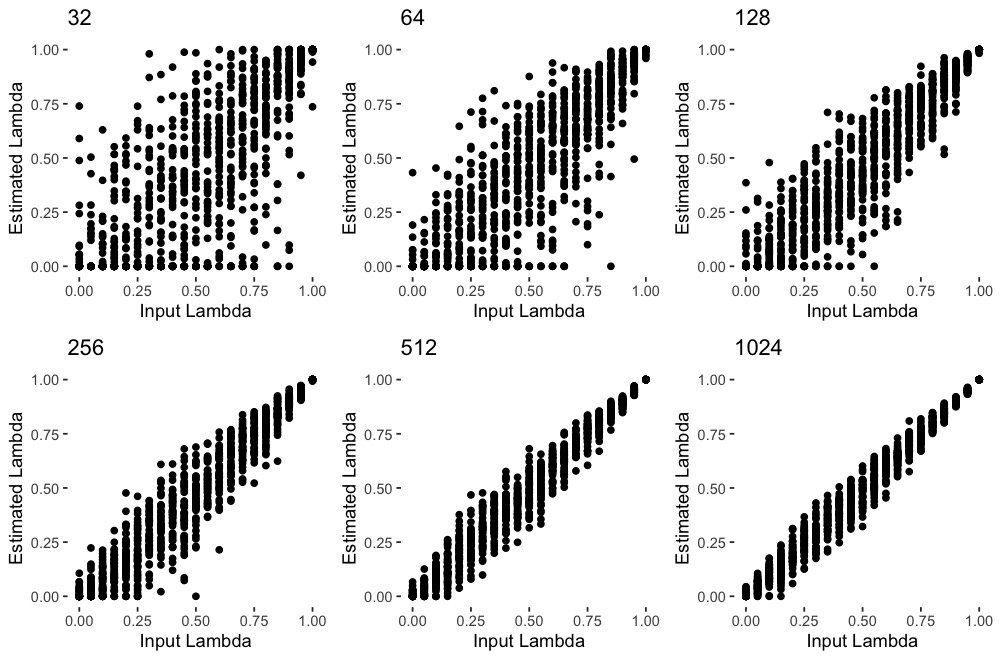
\includegraphics[width=0.95\linewidth]{Fig1}

\singlespacing \textbf{Figure 1}. Frequency distribution of \(\lambda\)
estimates published in 2019. The majority of these values were close to
0 or 1, and from phylogenies with fewer than 200 taxa.

\newpage

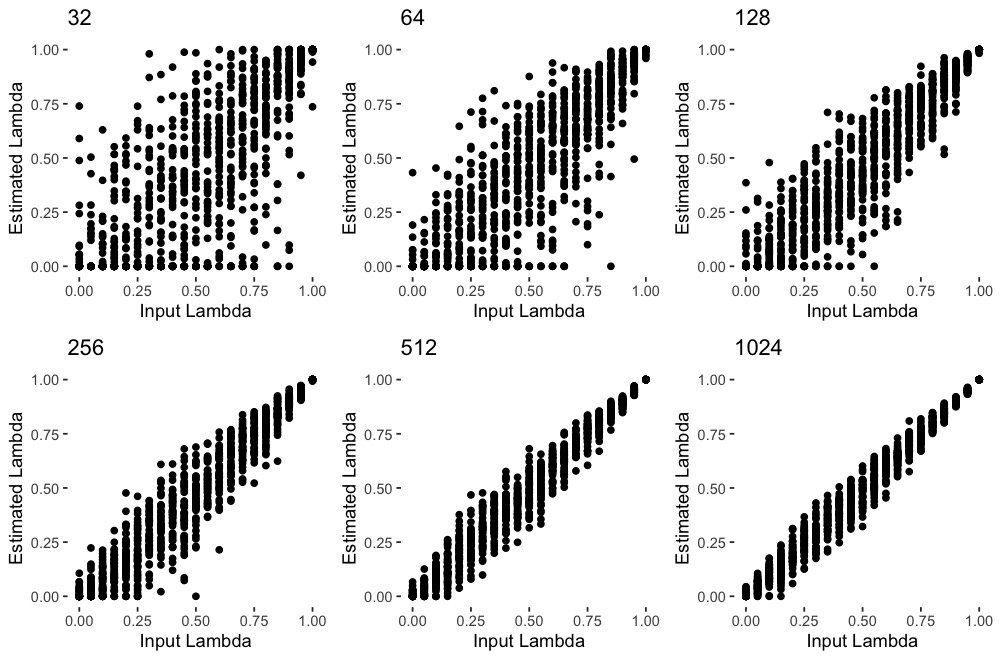
\includegraphics[width=0.95\linewidth]{Fig2}

\singlespacing \textbf{Figure 2}. Precision of Pagel's \(\lambda\)
across known levels of input phylogenetic signal (\(\lambda_{in}\)) on
phylogenies of various sizes. As phylogenies increase in size, variation
in \(\lambda_{in}\) decreases; however the precision is not constant
across the range of input levels (\(\lambda_{in}: 0 \to 1\)), and is
highest at intermediate levels of phylogenetic signal.

\newpage

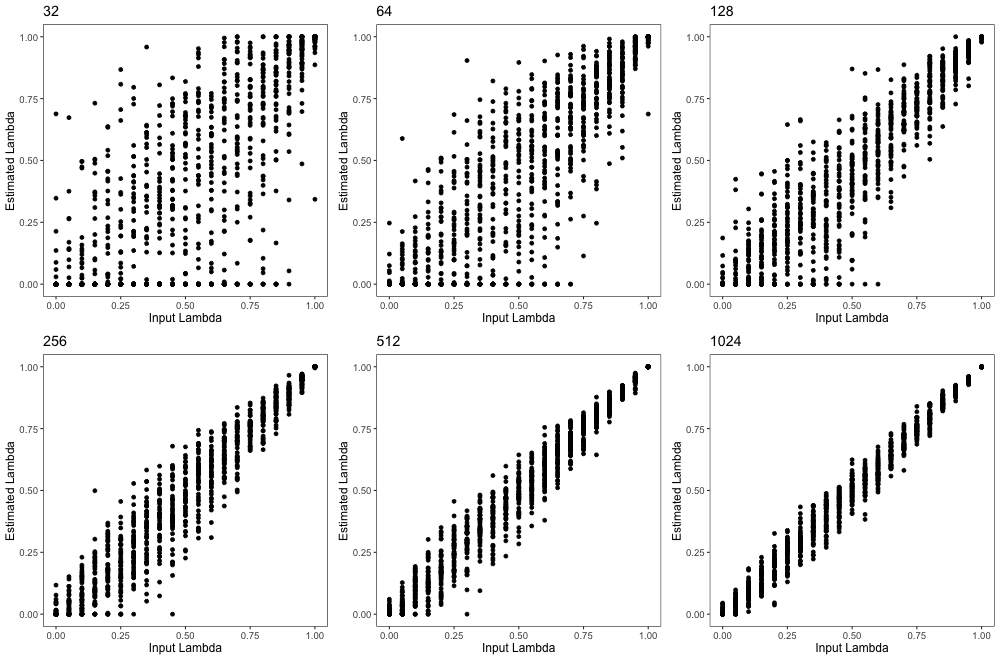
\includegraphics[width=0.95\linewidth]{Fig3}

\singlespacing \textbf{Figure 3}. Precision of Pagel's \(\lambda\) when
incorporated in phylogenetic regression (\(Y\sim X\)), across known
levels of input phylogenetic signal (\(\lambda_{in}\)) on phylogenies of
various sizes. As phylogenies increase in size, variation in
\(\lambda_{in}\) decreases; however the precision is not constant across
the range of input levels (\(\lambda_{in}: 0 \to 1\)), and is highest at
intermediate levels of phylogenetic signal.

\newpage

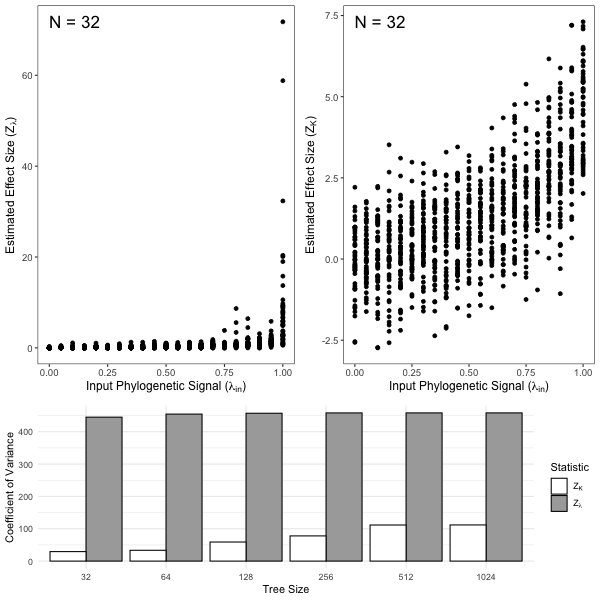
\includegraphics[width=0.95\linewidth]{Fig4}

\singlespacing \textbf{Figure 4}. Variation in effect size estimates of
phylogenetic signal across input levels of phylogenetic signal. (A)
Estimates \(Z_\lambda\) for data simulated on phylogenies with 32 taxa
(\(n=32\)), (B) Estimates of \(Z_\kappa\) for data simulated on
phylogenies with 32 taxa (\(n=32\)), (C) Coefficients of variation of
precision estimates of \(Z_\lambda\) and \(Z_\kappa\) across input
levels of phylogenetic signal, estimated on phylogenies containing
differing numbers of species.

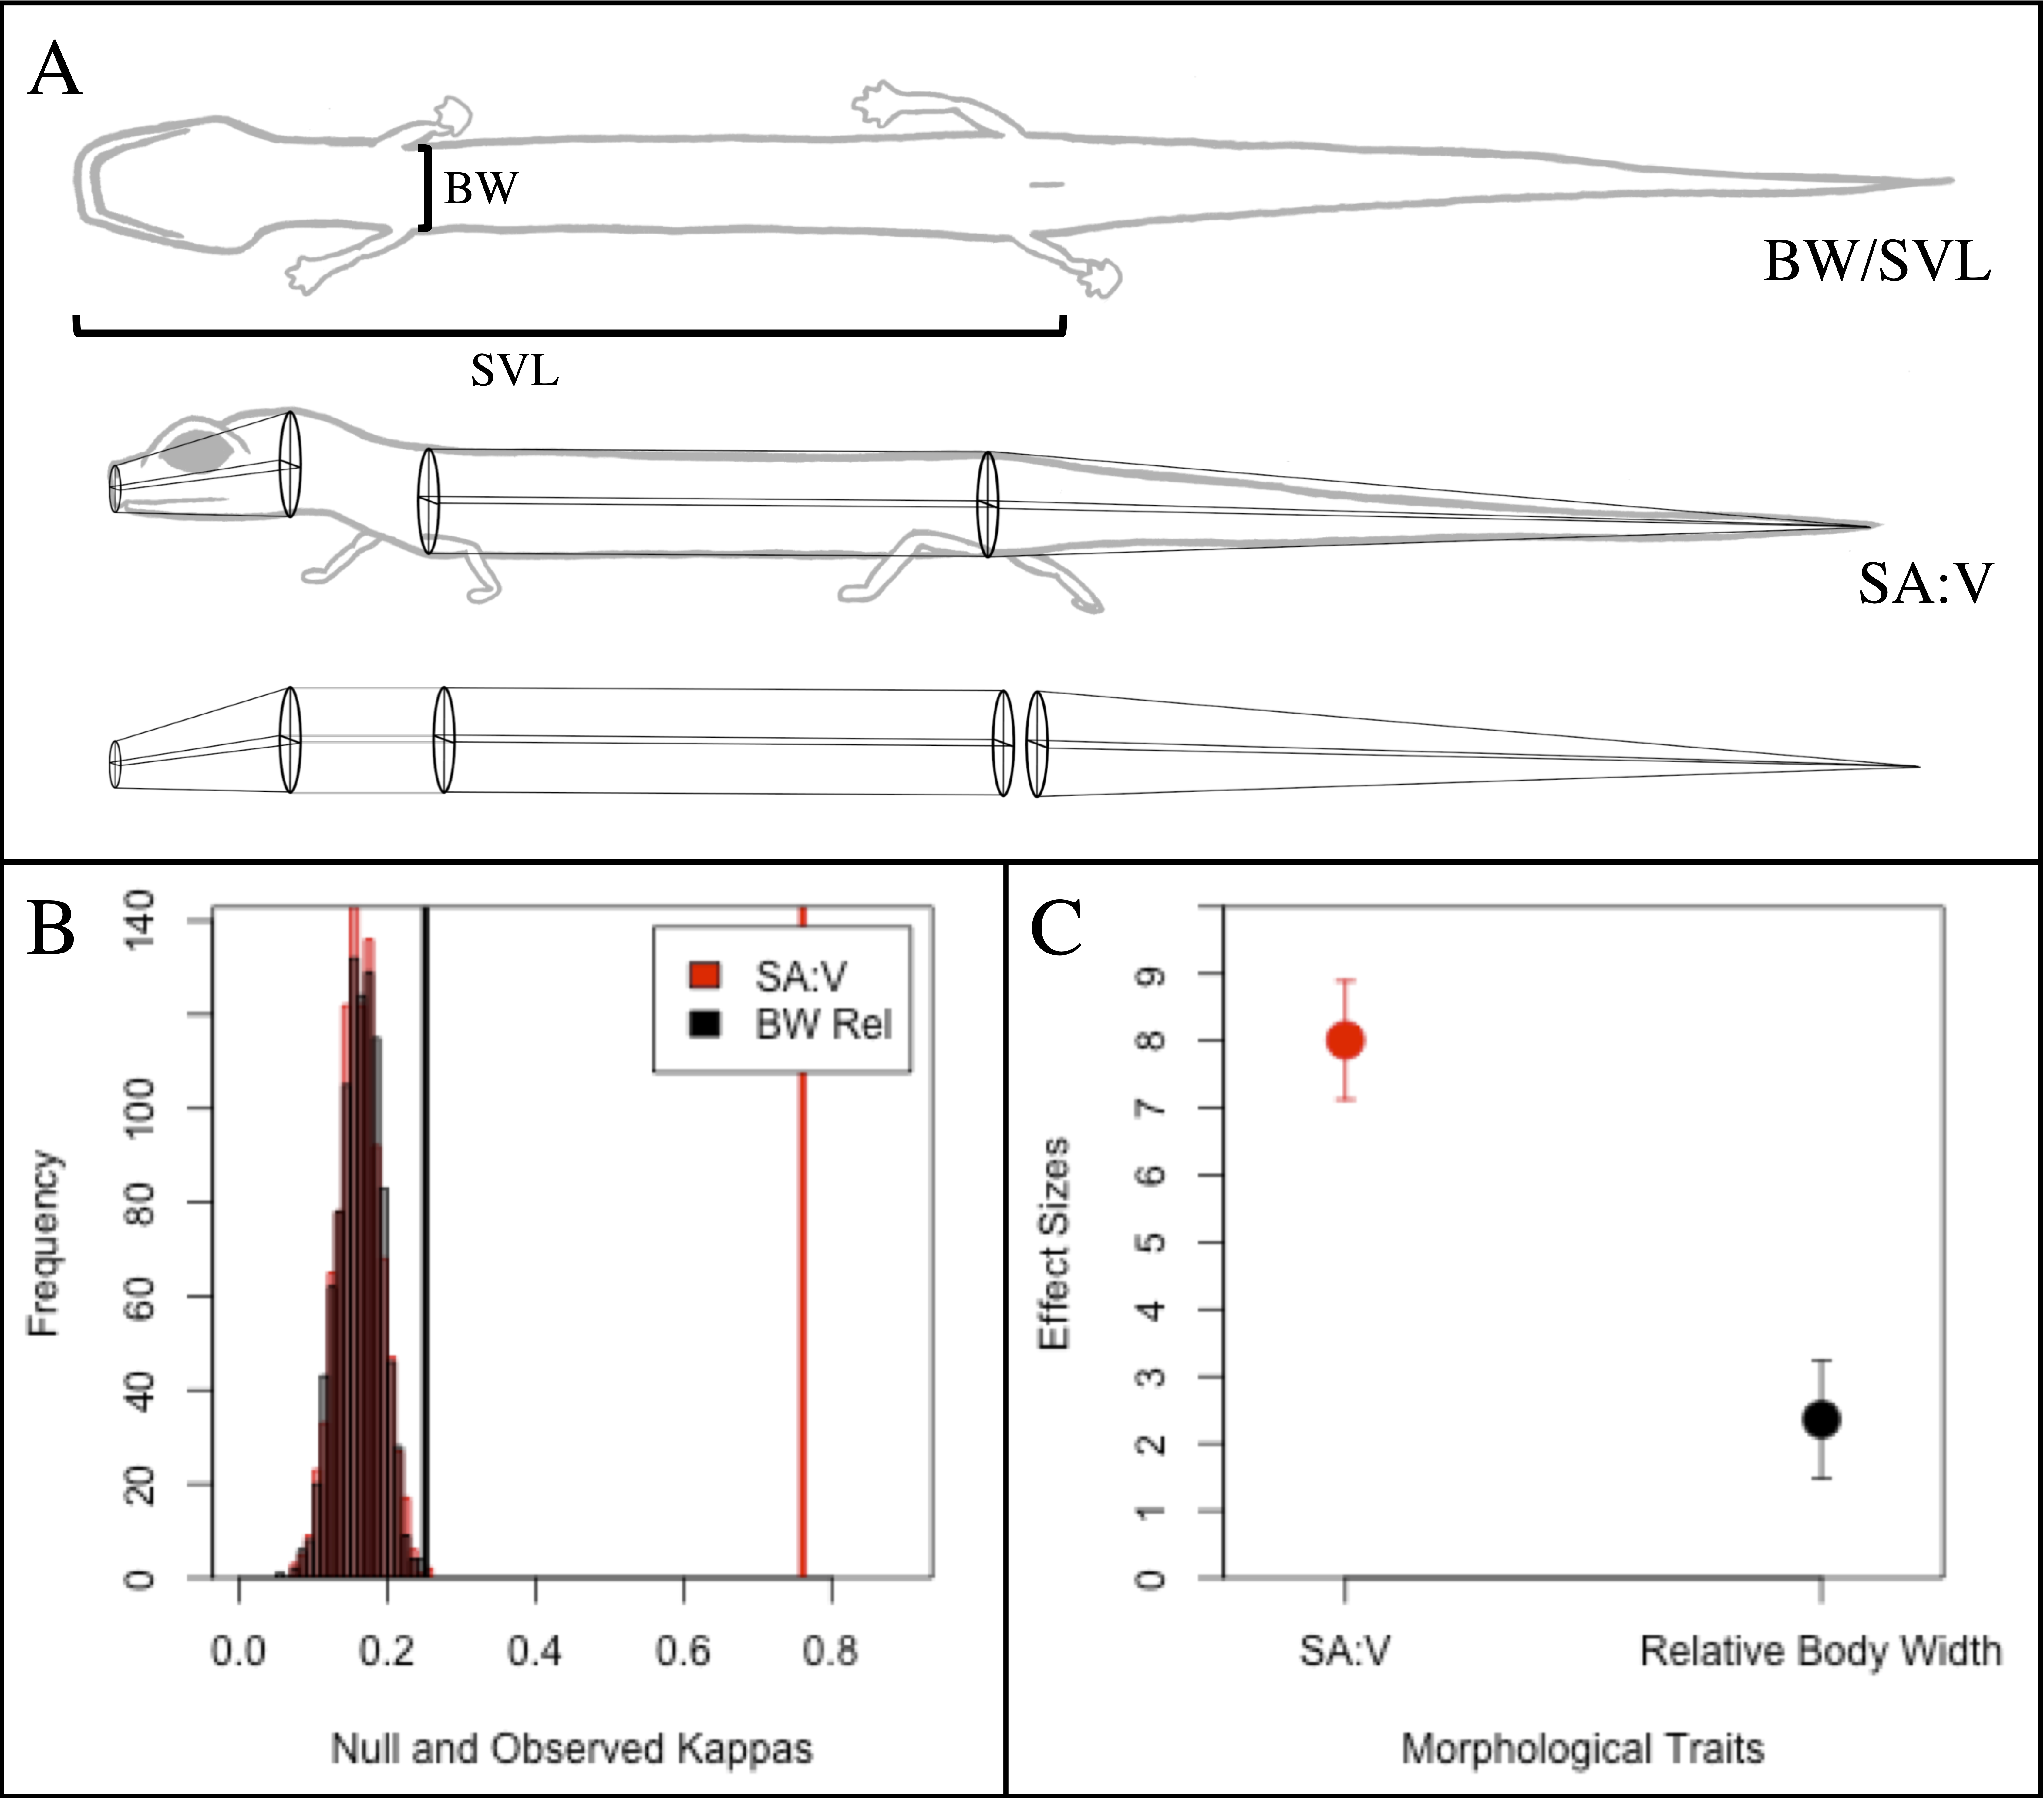
\includegraphics[width=0.95\linewidth]{Fig5}

\singlespacing \textbf{Figure 5}. (A) Linear measures for relative body
size, and regions of the body used to estimate surface area to volume
(SA:V) ratios. (B) Permutation distributions of phylogenetic signal for
SA:V and \(\frac{BW}{SVL}\), with observed values shown as vertical
bars. (C) Effect sizes (\(Z_\kappa\)) for SA:V and \(\frac{BW}{SVL}\),
with their 95\% confidence intervals (CI not standardized by
\(\sqrt(n)\)).

\end{document}
